\documentclass[11pt]{beamer}
\usetheme{Berkeley}
\setbeamertemplate{navigation symbols}{}%remove navigation symbols
% \usepackage{cogsci}
% \usepackage{fullpage}
\usepackage{booktabs}
\usepackage{pslatex}
\usepackage{apacite}
\usepackage{amsmath}
\usepackage{subcaption}
\usepackage{pgfplots}
\usepackage{wrapfig}
\usepackage{graphicx}
% \usepackage{url}
% \usepackage{hyperref}
% \usepackage{bigfoot}
% \usepackage[export]{adjustbox}
% \setlength\intextsep{0pt}

\AtBeginSection[]{
  \begin{frame}
  \vfill
  \centering
  \begin{beamercolorbox}[sep=8pt,center,shadow=true,rounded=true]{title}
    \usebeamerfont{title}\insertsectionhead\par%
  \end{beamercolorbox}
  \vfill
  \end{frame}
}

\usepackage{graphicx}

\usepackage{gb4e}  % linguistic examples
\noautomath

\title[]{The impact of parameterizations and assumptions on a model of opinion dynamics}
\author[M.~A.~Turner]{
  {Matthew~A.~Turner}
}
\date{\today}

\begin{document}
\maketitle

\begin{frame}{Outline}
  \begin{enumerate}
    \item Flache and Macy (2011) model of opinion dynamics\footnote{Flache, A., \& Macy, M. W. (2011). Small Worlds and Cultural Polarization. The Journal of Mathematical Sociology, 35(1–3), 146–176.}
    \item A few notes on the big, confusing field of opinion/social/cultural
      dynamics and polarization
    \item The impact of parameterizations and assumptions: room to explore
      \begin{itemize}
        \item Initial conditions
        \item Noisy opinion updating
        \item The interpretation of zero opinions and rules for influence
        \item Dynamics under increasing ``cultural complexity''
      \end{itemize}
  \end{enumerate}
\end{frame}

\section{Introduction}

\begin{frame}{Motivation}
  Polarization is a necessarily ``big'' concept. There are many models of it to serve many 
  purposes. 
  \\[1em]
  It's important because the media we consume (cable news, internet news, and
  social media) is widely consumed and ideologically driven \cite{Pew2014}.
  \\[1em]
  We formulate our opinions based on such info, so it's important to understand
  how this information can deepen or bridge interpersonal division. We can
  learn how others became divided or not based on their utterances on
  social media \cite{Borge-Holthoefer2014, Morales2015a}.
  \\[1em]
  Large social surveys can enable large-scale, more precise measurements of
  polarization.  
\end{frame}

\begin{frame}{Motivation, continued}
  I am interested in how the concepts we use in communication
  affect cognition in social and cultural settings. 
  \\[1em]
  A preliminary step that is not yet
  well-understood is just to answer how perfectly-transmitted
  and understood conceptual organizations can affect agents connected on a 
  social network.
  \\[1em]
  ``Conceptual organizations'' in this model are represented for each agent
  as a vector of ``opinions'' on a set of cultural features.
\end{frame}

\begin{frame}{Our contribution}
  We ask of this model, ``which parameterizations lead to 
  polarizing behavior, and which lead to global consesus?'' 
  \\[1em]
  We investigate what impact noisy opinion updating has on polarization
  dynamics.
  \\[1em]
  We consider the impact of the choice of disagreement measure for different
  cultural complexities.
\end{frame}

% \begin{frame}{Motivating questions}
%   But what is polarization and under what conditions does it
%   emerge? 
%   \\[1em]
%   Is there hope for a common framework for understanding the dynamics
%   of opinion updating, which in some cases results in polarization?
% \end{frame}

\subsection{Flache and Macy (2011) model of ``cultural polarization''}

\begin{frame}{Agent-based model}
  Agents are nodes in a \emph{small-world} graph\footnote{Watts, D. J. J., \& Strogatz, S. H. H. (1998). Collective dynamics of “small-world” networks. Nature, 393(6684), 440–442. http://doi.org/10.1038/30918}. Neighboring agents
  directly influence a focal agent.
\\[1em]
Large increases in average path length from randomization cannot be
detected locally.
\end{frame}
\begin{frame}{Illustration of building small-world network (1 of 2)}

  \begin{figure}[t!]
    \centering
        % \begin{subfigure}[t]{0.5\textwidth}
            % \centering
            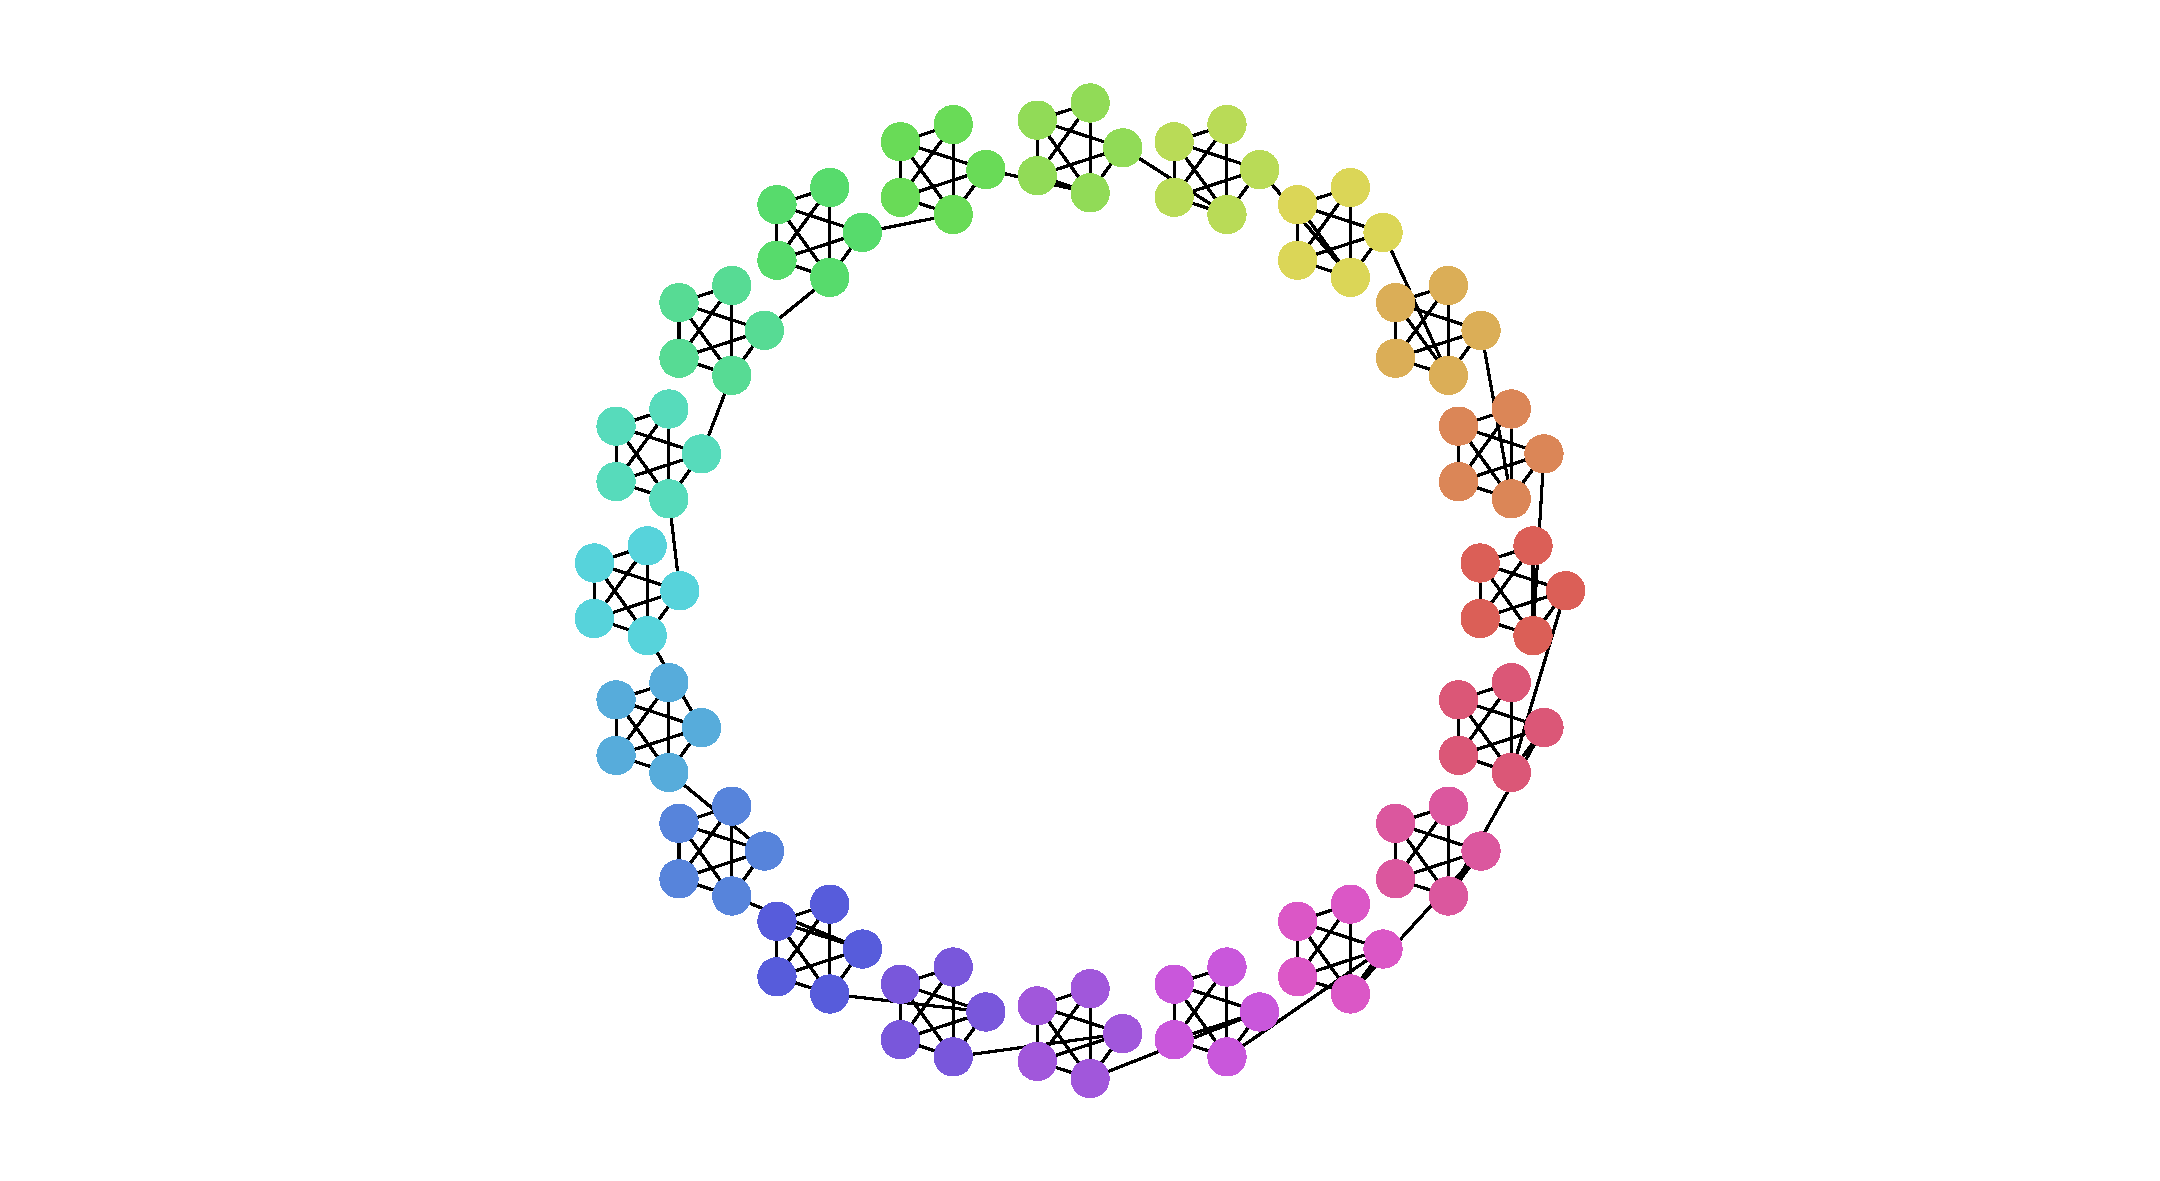
\includegraphics[width=\textwidth]{Figures/n=20-k=5-norandom.pdf}
            \caption{Connected caveman network before random ties added.
              20 ``caves'' with 5 agents per cave.
            }
        % \end{subfigure}
        % \begin{subfigure}[t]{0.5\textwidth}
        \end{figure}
\end{frame}
  \begin{frame}{Illustration of building a small-world network (2 of 2)}
  \begin{figure}[t!]
            \centering
            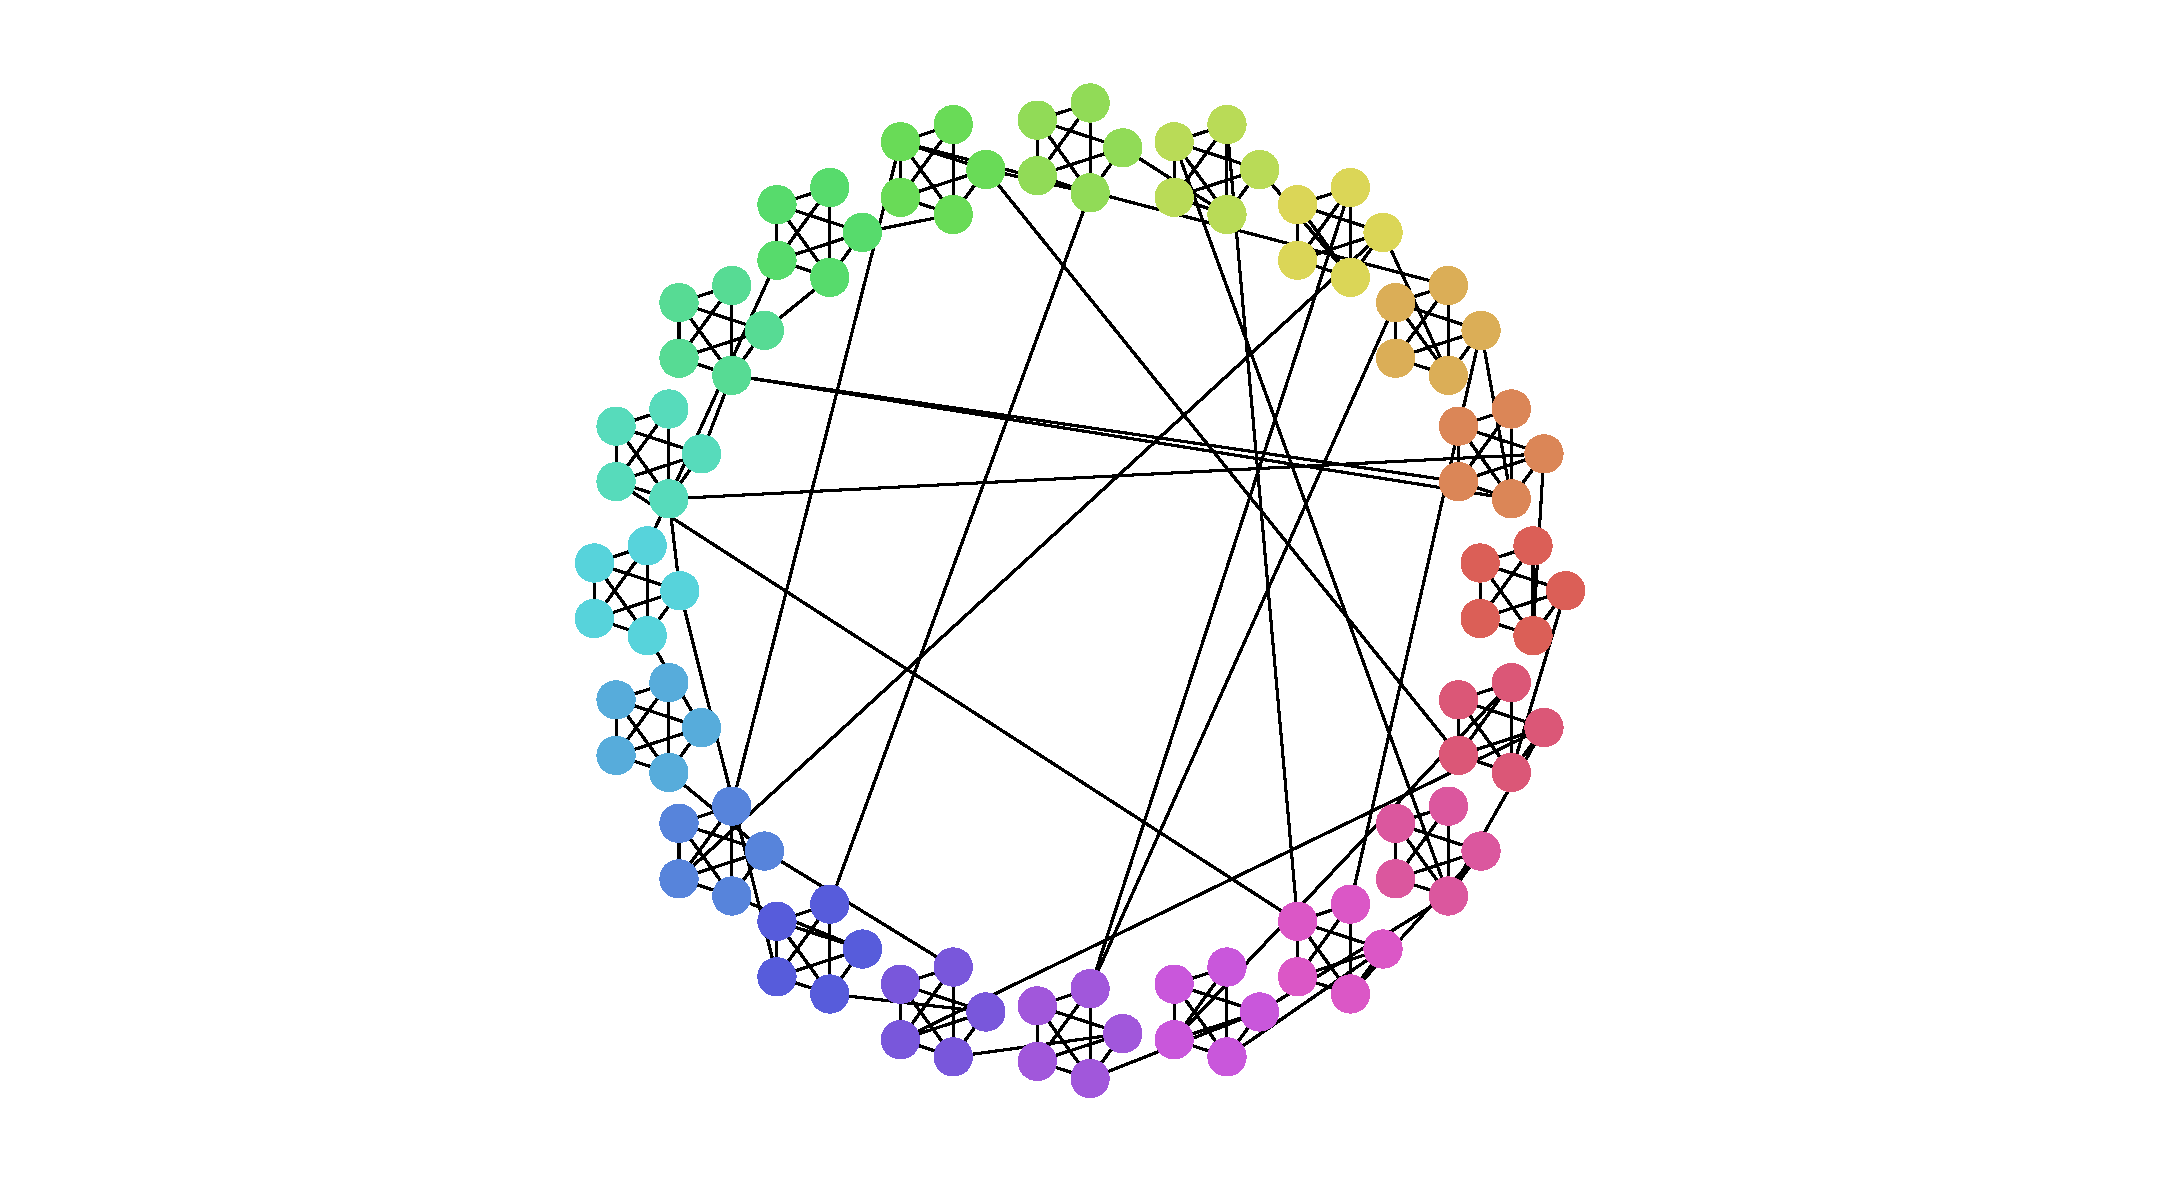
\includegraphics[width=\textwidth]{Figures/n=20-k=5-20random.pdf}
            \caption{Connected caveman network after 20 random ties added.}
        % \end{subfigure} 
        % \caption{Begin with connected caveman network, where one agent of each
        %   cave is connected to the next cave counter-clockwise.
        % }
        % \label{fig:cool}
    \end{figure}
\end{frame}

\begin{frame}{Agent opinions are vectors}
  Agents have $K$ opinions on a set of cultural features. $K$ is called the
  \emph{cultural complexity}. Final polarization, defined later, is 
  sensitive to cultural complexity in the Flache and Macy (2011) model. 
  \\[1em]
  Agent $i$ then has an opinion on each cultural feature, represented as an
  \emph{opinion vector}.
  \[
    s_i = \begin{pmatrix}
      s_{i0} \\
      \vdots \\
      s_{iK}
    \end{pmatrix}
  \]
  There is an implicit time dependence in agent opinion vectors, and thus
  in all other quantities derived from agent opinions.
  \\[1em]
  \[
    |s_{ik}| \leq 1 \quad \forall i, k
  \]
\end{frame}

\begin{frame}{Agent disagreement}
  In Flache and Macy (2011), disagreement, i.e.\ opinion distance, between two
  agents $i$ and $j$ is defined as
  \[
    d_{ij} = \frac{1}{K} \sum_{k=1}^K \lvert s_{jk} - s_{ik} \rvert.
  \]
  In words: opinion distance is the average of absolute opinion feature
  differences between the agents.
\end{frame}

\begin{frame}{Attractive or repulsive relationship?}
  Whether or not agents in a dyad are attracted to or repelled from each other
  depends on the extent of their disagreement. Define the attraction in
  terms of an edge weight, which can be between -1 and 1
  \[
    w_{ij} = 1 - d_{ij}
  \]
  Negative weights indicate a repulsive relationship. Attractive relationships
  obtain whenever $d_{ij} < 1$.
\end{frame}

\begin{frame}{Opinion updating}
  Away from the edges of opinion space, agent opinion features
  are updated by a value
  \[
    \Delta s_{ik} = \frac{1}{2 N_i}\sum_{i \neq j} w_{ij} \left( s_{jk} - s_{ik} \right)
  \]
  $N_i$ is the number of neighbors of agent $i$. So this is the average of 
  all neighbor ``forces'' on agent $i$.
  \\[1em]
  To constrain opinions $|s_{ik}| \leq 1$, this update value is smoothed when
  updating the opinion features themselves:

  \[
    s_{ik,t+1} = \begin{cases}
      s_{ik,t} + \Delta s_{ik,t}(1 - s_{ik,t}) & \text{ if} \quad s_{ik,t} > 0 \\
      s_{ik,t} + \Delta s_{ik,t}(1 + s_{ik,t}) & \text{ if} \quad s_{ik,t} \leq 0
    \end{cases}
  \]
\end{frame}

\begin{frame}{Outcome measure: polarization}
  \[
    P = \text{var}(d_{ij})
  \]
\end{frame}

\section{Experiments}

\begin{frame}{Average of trials with $K=2$}
\begin{figure}
  \centering
  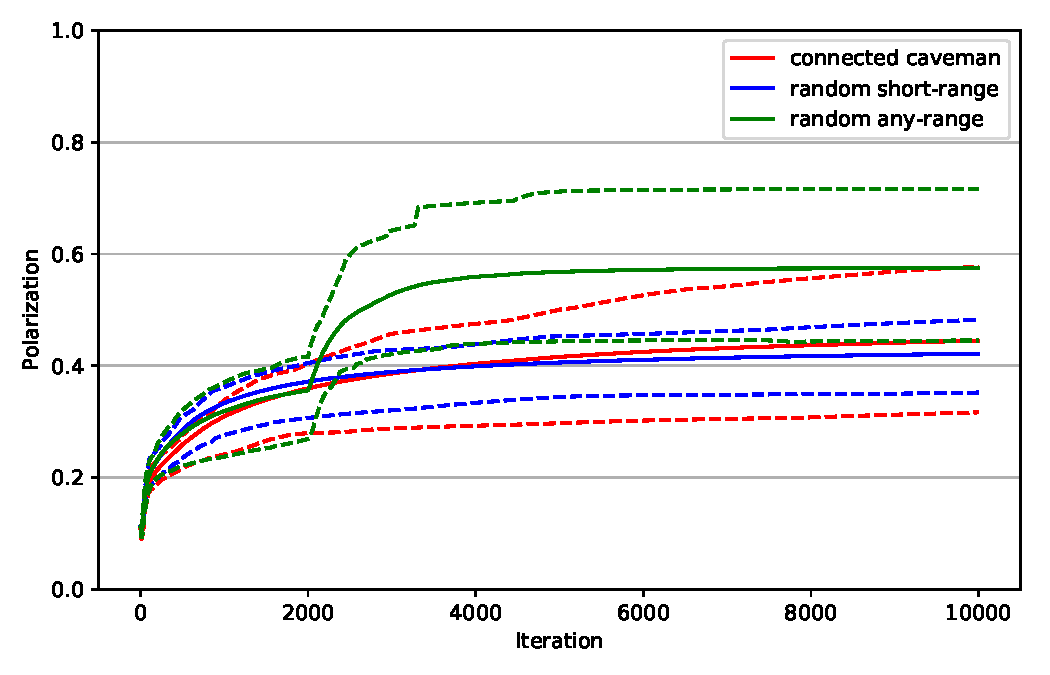
\includegraphics[width=\textwidth]{Figures/figure10b.pdf}
\end{figure} 
\end{frame}

\subsection{Initial conditions}

\begin{frame}{Initial conditions}

  In Flache and Macy (2011), every $s_{ik,t=0}$ is drawn from a uniform random
  distribution on $[-1, 1]$. Our first experiment considers initial opinion
  features drawn instead from $[-S, S]$, where $-1 \leq S \leq 1$.
  \begin{figure}
    \centering
    \includegraphics[width=\textwidth]{initial-opinion-example.pdf}
  \end{figure}
\end{frame}

\begin{frame}{Initial conditions}
  \begin{figure}
    \centering
    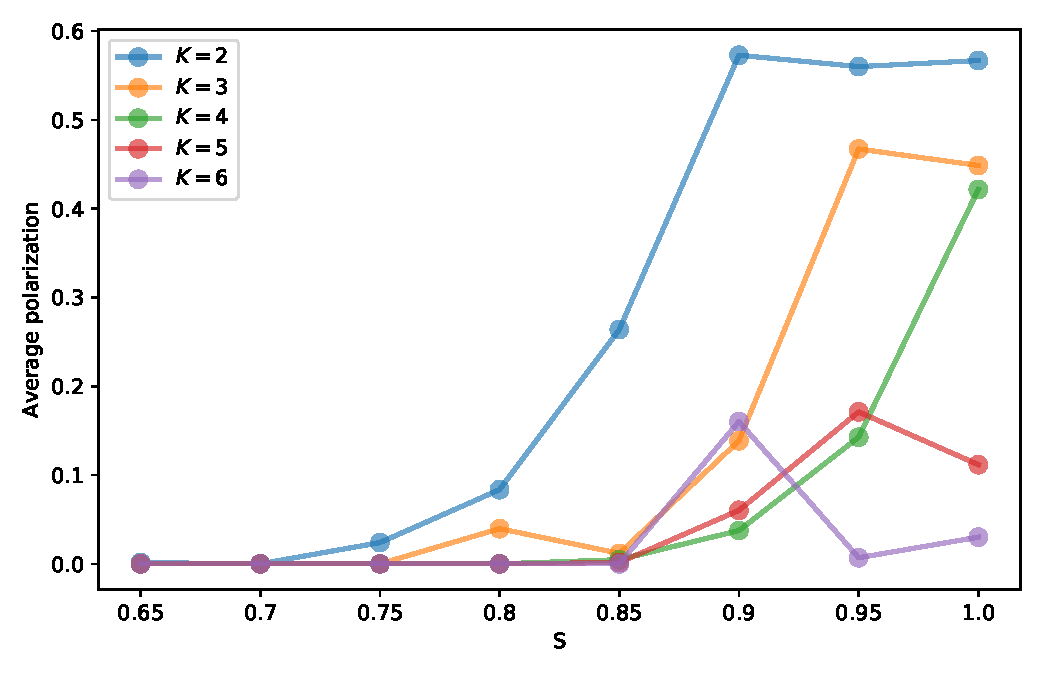
\includegraphics[width=\textwidth]{Figures/P_vs_S_for_K.pdf}
    \label{fig:p_vs_s_for_k}
  \end{figure}
\end{frame}

\subsection{Noisy updates}

\begin{frame}{Noisy updates}
  We add a noise term to the updates for each opinion feature. That is, modify
  \[
    \Delta s_{ik} = \frac{1}{2 N_i}\sum_{i \neq j} w_{ij} \left( s_{jk} - s_{ik} \right)
  \]
  to be
  \[
    \Delta s_{ik} = \frac{1}{2 N_i}\sum_{i \neq j} w_{ij} \left( s_{jk} - s_{ik} \right) + \epsilon
  \]
  where $\epsilon \sim  \mathcal{N} (0, \sigma)$. We vary $\sigma$, which we
  call the \emph{noise level}.
\end{frame}

\begin{frame}{Noisy updates}
  \begin{figure}[t!]
    \centering
        \begin{subfigure}[t]{0.49\textwidth}
            \centering
            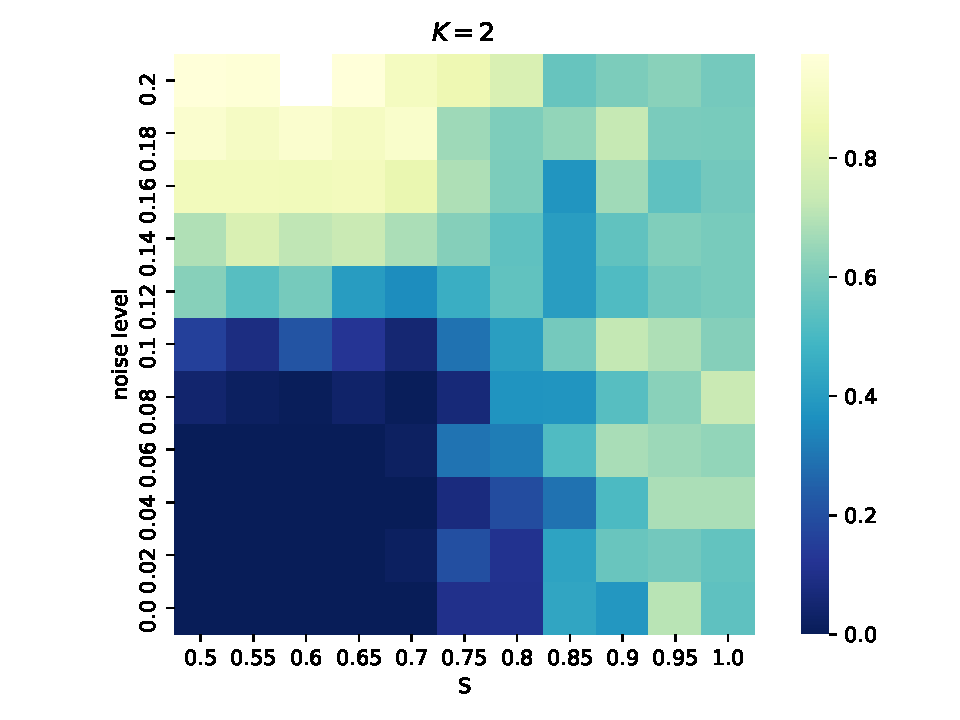
\includegraphics[width=0.9\textwidth]{Figures/p_v_noise_k=2.pdf}
        \end{subfigure}
        \begin{subfigure}[t]{0.49\textwidth}
            \centering
            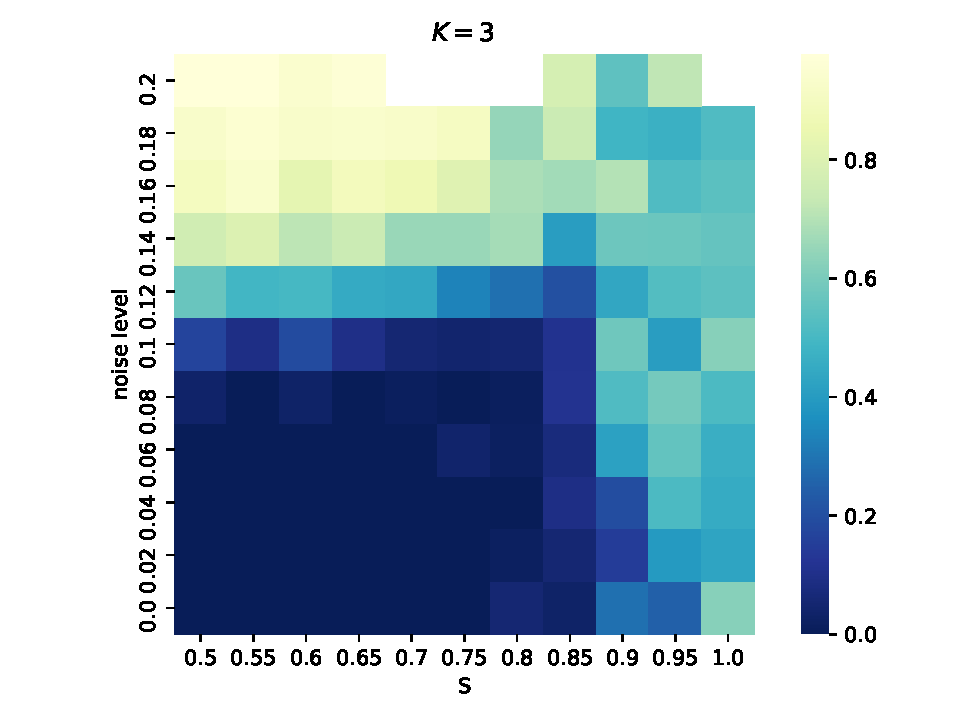
\includegraphics[width=0.9\textwidth]{Figures/p_v_noise_k=3.pdf}
        \end{subfigure} \\
    \begin{subfigure}[t]{0.49\textwidth}
        \centering
        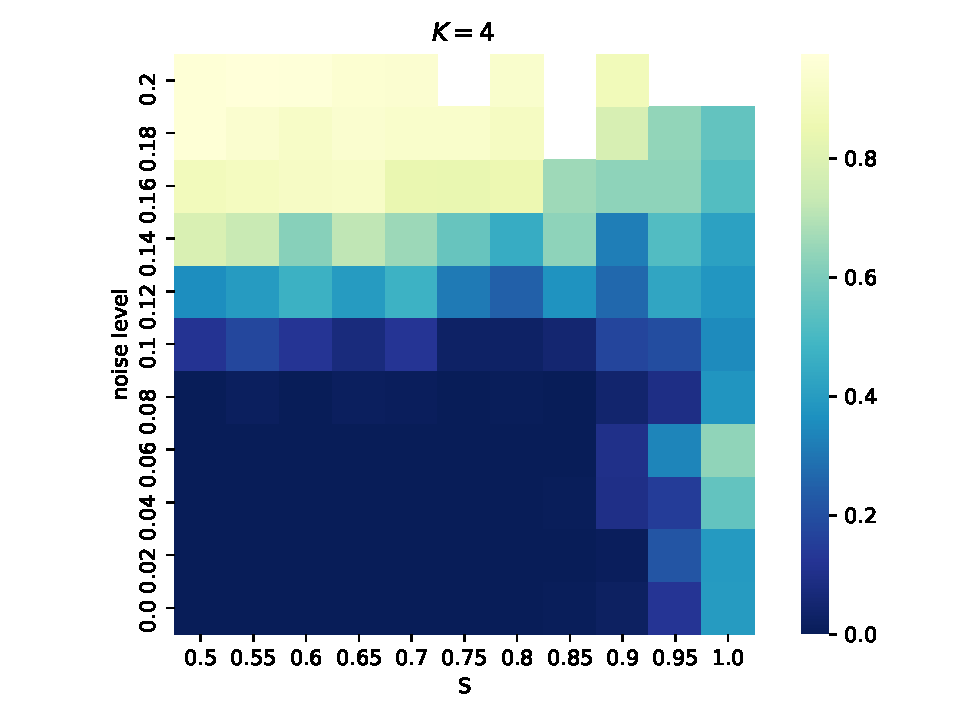
\includegraphics[width=0.9\textwidth]{Figures/p_v_noise_k=4.pdf}
    \end{subfigure}
    \begin{subfigure}[t]{0.49\textwidth}
        \centering
        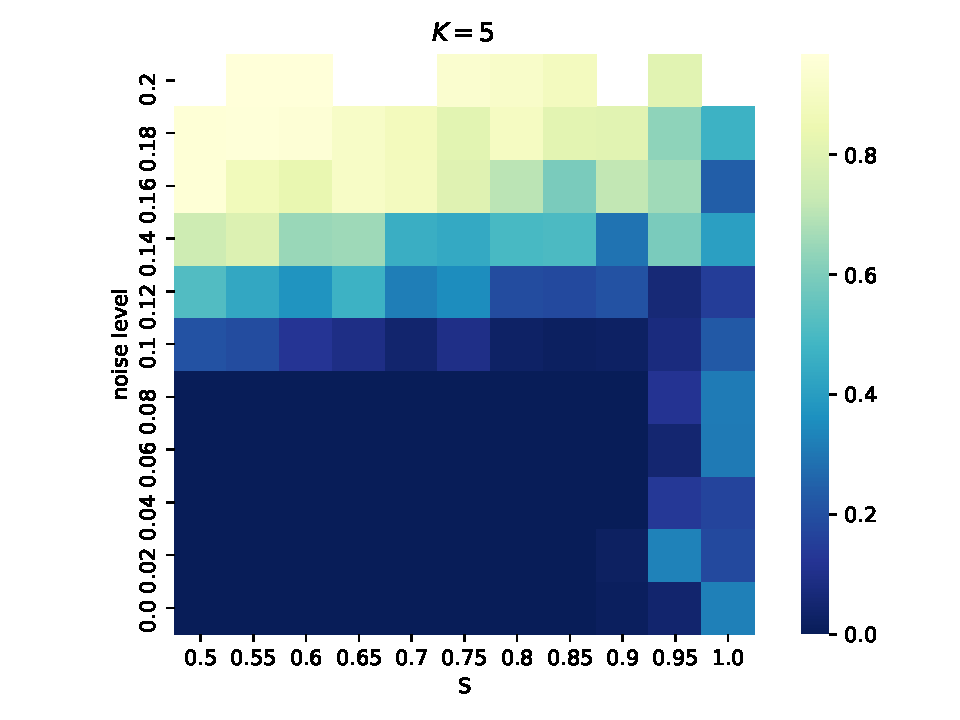
\includegraphics[width=0.9\textwidth]{Figures/p_v_noise_k=5.pdf}
    \end{subfigure}
    \label{fig:heatmaps}
  \end{figure}
\end{frame}

\begin{frame}{Final polarization as a function of cultural complexity}
  \begin{figure}
    \centering
        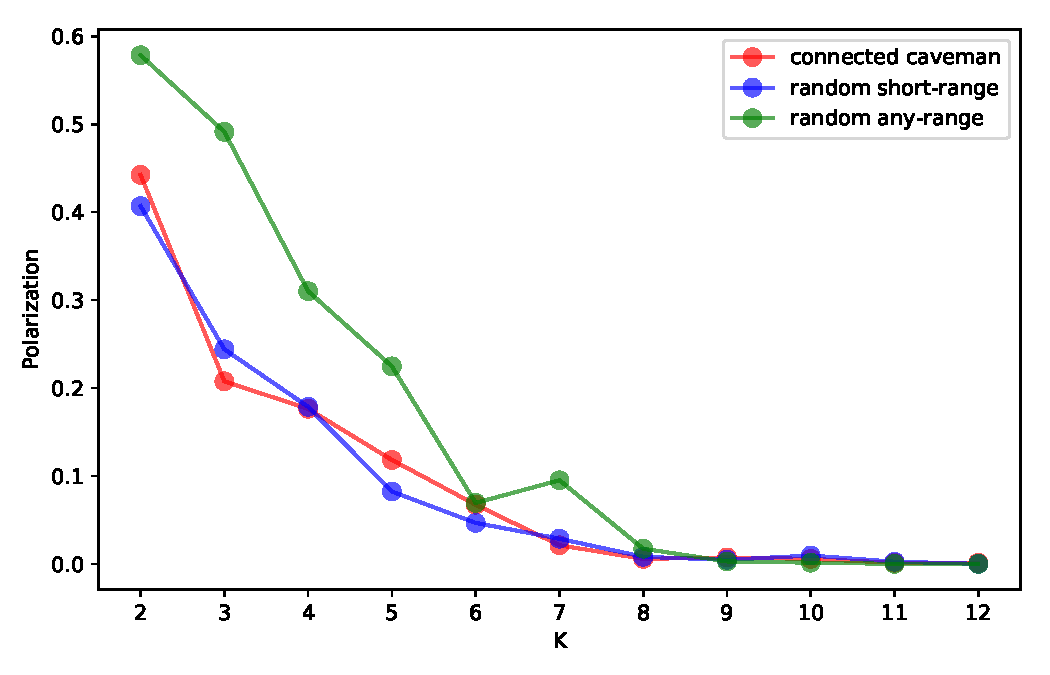
\includegraphics[width=\textwidth]{Figures/finegrained_p_vs_K.pdf}
    % \caption{
    %   Compare to FM 2011 Figure 12b. Identical, but with more intermediate
    %   values of cultural complexity $K$. As found by Flache and Macy, 
    %   average final polarization decreases with $K$. Each
    %   data point is the average of fifty trials. Each trial ran over 
    %   10k timesteps.
    % }
    \label{fig:k_finegrained}
  \end{figure}
\end{frame}

\begin{frame}{Three ``phase transitions''}
  \begin{enumerate}
    \item Maximum initial opinion magnitude
    \item Magnitude of noise in noisy updates
    \item Cultural complexity
  \end{enumerate}
\end{frame}

\begin{frame}{Three ``phase transitions''}
  \begin{enumerate}
    \item Maximum initial opinion magnitude
    \item Magnitude of noise in noisy updates
    \item \textbf{Cultural complexity}
  \end{enumerate}
\end{frame}

\subsection{Alternative distance measure?}

\begin{frame}{Should shared irrelevance be attractive?}
  In the original Flache and Macy (2011) model, two opinions of 0 on a
  cultural feature count as agreement on that feature. This seems reasonable
  enough, but it could be argued that in other situations, agreement on
  irrelevance would not increase attraction between two agents.
  \\[1em]
  No empirical support for this assumption in Flache and Macy (2011).
\end{frame}

\begin{frame}{Cosine distance as an alternative}
  Defined as 
  \[
    d_{ij} = 1 - \frac{s_i \cdot s_j}{\lVert s_i \rVert \lVert s_j \rVert}
  \]
  then
  \[
    w_{ij} = \frac{s_i \cdot s_j}{\lVert s_i \rVert \lVert s_j \rVert}.
  \]
  Attraction occurs when the angle between agents is less than $\pi/2$ and
  repulsion when the angle is greater than $\pi / 2$.
\end{frame}

\begin{frame}{Initial conditions with cosine distance}
  \begin{figure}
    \centering
    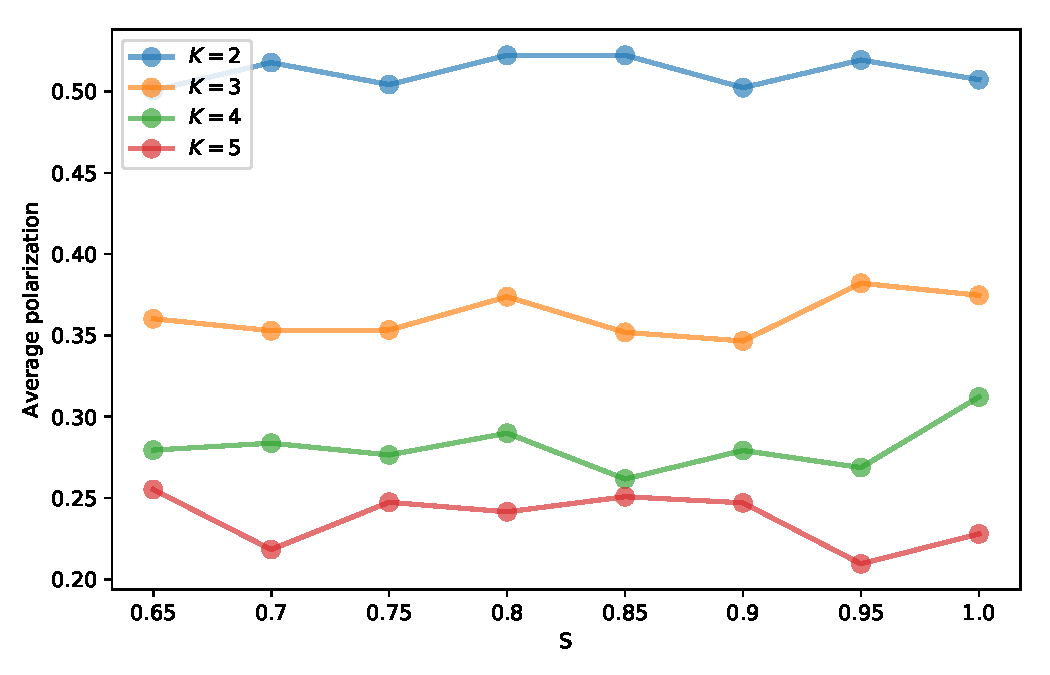
\includegraphics[width=\textwidth]{Figures/P_vs_S_for_K_cosine.pdf}
    \label{fig:p_vs_s_for_k}
  \end{figure}
\end{frame}

\begin{frame}{Noisy updates with cosine distance}
  \begin{figure}[t!]
    \centering
        \begin{subfigure}[t]{0.49\textwidth}
            \centering
            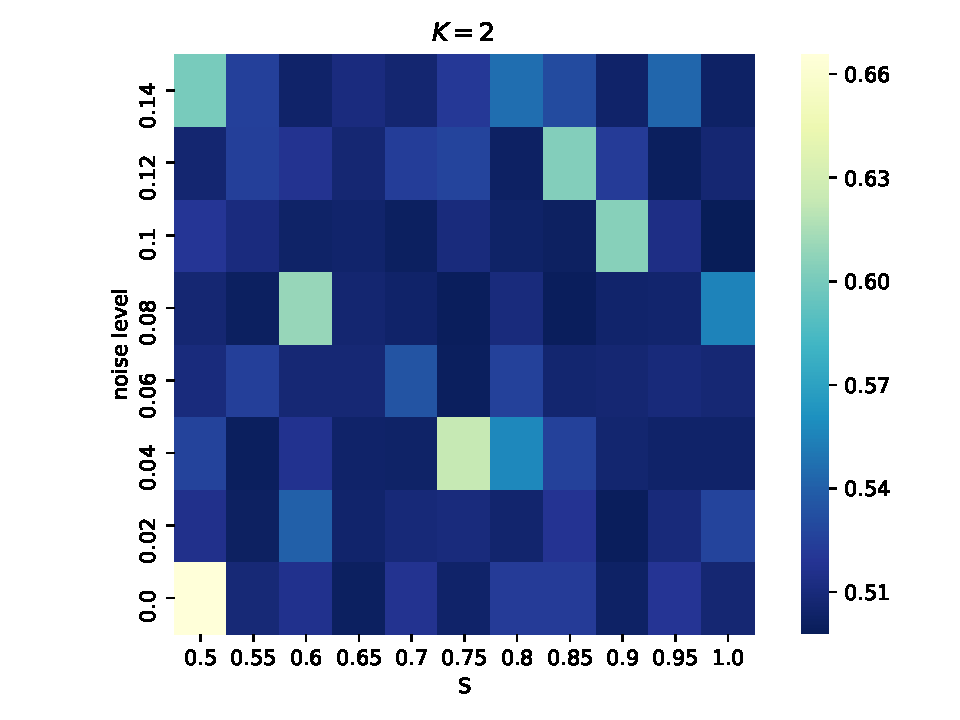
\includegraphics[width=0.9\textwidth]{Figures/p_v_noise_k=2_cosine_distance.pdf}
        \end{subfigure}
        \begin{subfigure}[t]{0.49\textwidth}
            \centering
            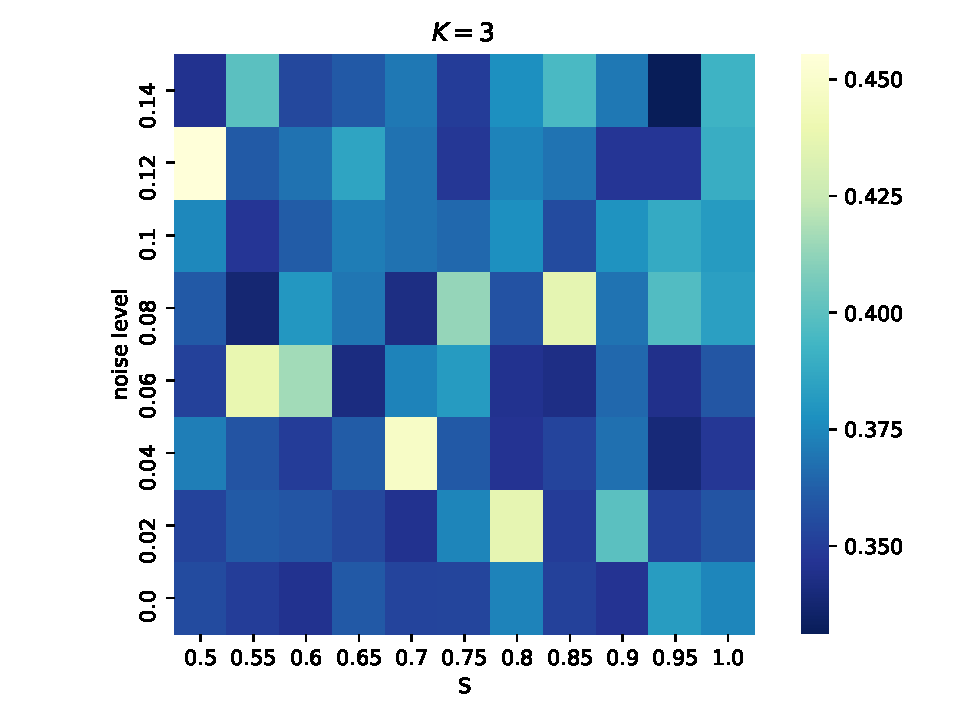
\includegraphics[width=0.9\textwidth]{Figures/p_v_noise_k=3_cosine_distance.pdf}
        \end{subfigure} \\
    \begin{subfigure}[t]{0.49\textwidth}
        \centering
        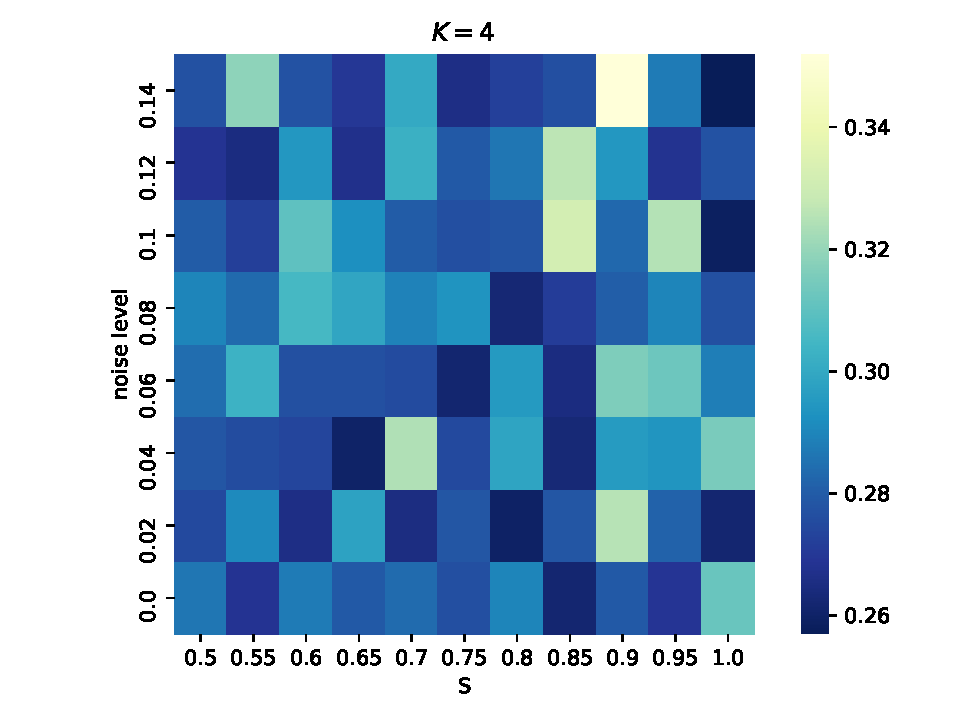
\includegraphics[width=0.9\textwidth]{Figures/p_v_noise_k=4_cosine_distance.pdf}
    \end{subfigure}
    \begin{subfigure}[t]{0.49\textwidth}
        \centering
        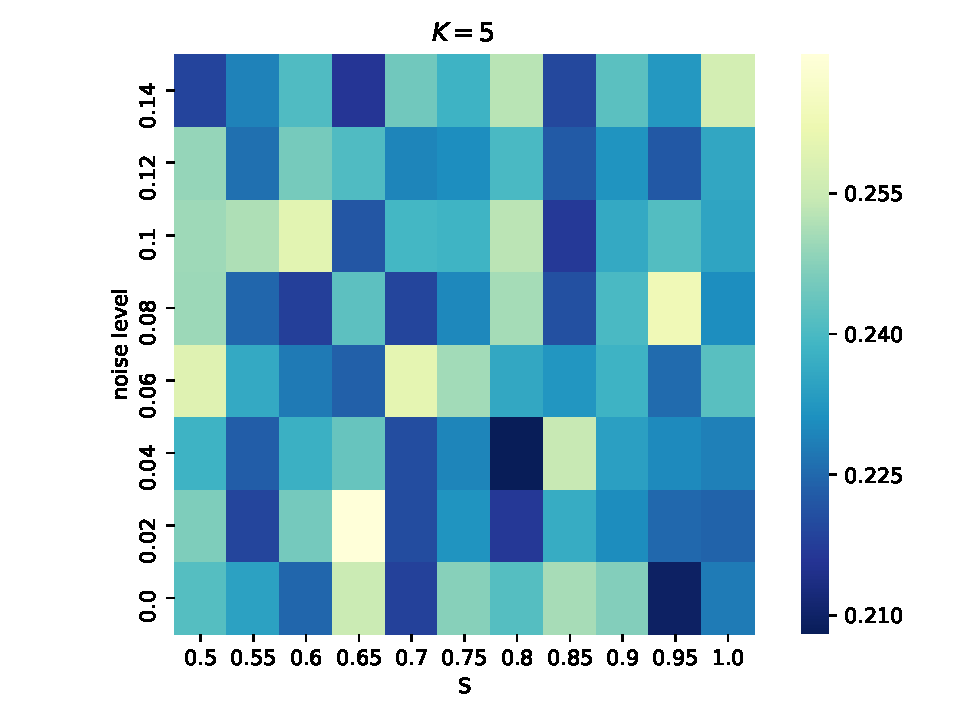
\includegraphics[width=0.9\textwidth]{Figures/p_v_noise_k=5_cosine_distance.pdf}
    \end{subfigure}
    \label{fig:heatmaps}
  \end{figure}
\end{frame}

\subsection{Exploring increasing cultural complexity}

\begin{frame}{Parallel coordinates}
  Use plots like this to explore whether polarization, as defined by 
  Flache and Macy (2011), is a useful measure. If not, what is?
  \begin{figure}
    \centering
    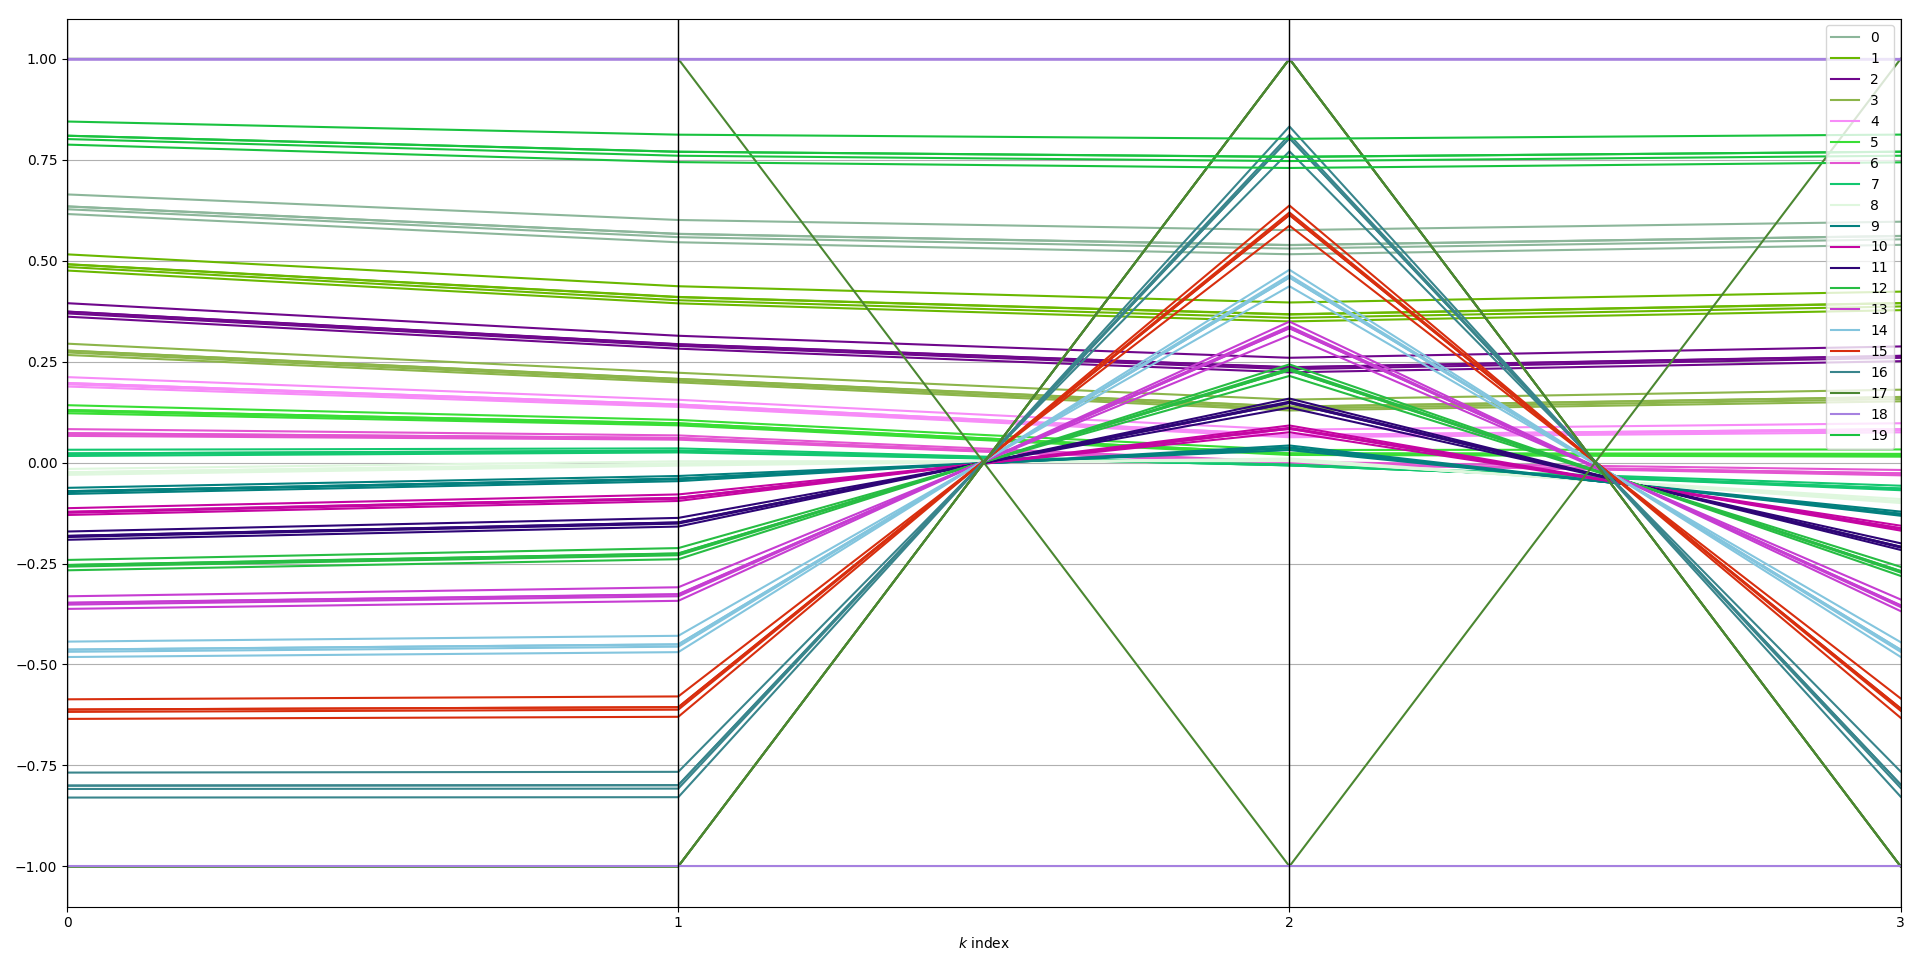
\includegraphics[width=0.8\textwidth]{parallel_coords_k=4.png}
  \end{figure}
\end{frame}

\begin{frame}{References}
\bibliographystyle{apacite}

\setlength{\bibleftmargin}{.125in}
\setlength{\bibindent}{-\bibleftmargin}

{\tiny
\bibliography{/Users/mt/workspace/papers/library.bib}
}
\end{frame}

\end{document}
